% ============================================================
% Plantilla de Documento Técnico - Trabajo Terminal
% Escuela Superior de Cómputo (ESCOM) - IPN
% ============================================================
\documentclass[12pt,letterpaper]{report}

% ---------------------- IMPORTS / PAQUETES ----------------------
\usepackage[utf8]{inputenc}        % Codificación de entrada UTF-8
\usepackage[T1]{fontenc}           % Codificación de fuentes
\usepackage[spanish,es-tabla]{babel} % Idioma español (títulos, fechas, "Tabla" en vez de "Cuadro")
\usepackage{geometry}              % Márgenes de página
\usepackage{graphicx}              % Inserción de imágenes
\usepackage{xcolor}                % Colores
\usepackage{booktabs}              % Tablas de calidad profesional
\usepackage{longtable}             % Tablas que abarcan varias páginas
\usepackage{array}                 % Control avanzado de columnas en tablas
\usepackage{multirow}              % Celdas que abarcan varias filas
\usepackage{tabularx}              % Tablas con columnas de ancho ajustable
\usepackage{fancyhdr}              % Encabezados y pies de página personalizados
\usepackage{titlesec}              % Formato personalizado de títulos de capítulo/sección
\usepackage{tocloft}               % Personalización de índices (contenido, tablas, figuras)
\usepackage{enumitem}              % Listas personalizadas (para requerimientos, objetivos, etc.)
\usepackage{amsmath,amssymb}       % Símbolos y entornos matemáticos
\usepackage{caption}               % Personalización de leyendas de figuras/tablas
\usepackage{subcaption}            % Subfiguras
\usepackage{float}                 % Control de posicionamiento de flotantes (H)
\usepackage{pdfpages}              % Insertar páginas PDF completas (p. ej. carta responsiva escaneada)
\usepackage{setspace}              % Control de interlineado
\usepackage{indentfirst}           % Sangría en el primer párrafo de cada sección
\usepackage[export]{adjustbox}     % Ajuste adicional de imágenes
\usepackage{csquotes}              % Comillas contextuales para citas
\usepackage[backend=biber,style=ieee,sorting=none]{biblatex} % Referencias en formato IEEE
\usepackage{hyperref}              % Hipervínculos y marcadores en el PDF (cargar casi al final)
\usepackage[capitalize]{cleveref}  % Referencias cruzadas inteligentes (después de hyperref)
% ---------------------- CONFIGURACIÓN GENERAL ----------------------
\geometry{left=3cm, right=2.5cm, top=2.5cm, bottom=2.5cm}
\addbibresource{referencias.bib}   % Archivo .bib con las referencias (crear aparte)

% Colores institucionales (opcional, tono guinda IPN)
\definecolor{guindaipn}{RGB}{106,17,63}

% Formato de títulos de capítulo
\titleformat{\chapter}[display]
  {\normalfont\bfseries\Large\color{guindaipn}}
  {\chaptertitlename\ \thechapter}{20pt}{\Large}
\titlespacing*{\chapter}{0pt}{-20pt}{20pt}

% Encabezado y pie de página
\pagestyle{fancy}
\fancyhf{}
\renewcommand{\headrulewidth}{0.4pt}
\fancyhead[L]{\small Instituto Politécnico Nacional -- ESCOM}
\fancyhead[R]{\small\leftmark}
\fancyfoot[C]{\thepage}

% Interlineado 1.5 para el cuerpo del documento
\onehalfspacing

% Numeración de figuras/tablas por capítulo
\counterwithin{figure}{chapter}
\counterwithin{table}{chapter}

% Hipervínculos sin bordes de color llamativos
\hypersetup{
    colorlinks=true,
    linkcolor=black,
    citecolor=guindaipn,
    urlcolor=blue,
    pdftitle={Modelo de optimización de alineaciones mediante análisis de emparejamientos en la WNBA},
    pdfauthor={Ulises Abdiel Cabello Cardenas, Fernanda Madariaga Villanueva}
}

% ---------------------- DATOS DEL DOCUMENTO ----------------------
\newcommand{\tituloTT}{Modelo de optimización de alineaciones mediante análisis de emparejamientos en la WNBA}
\newcommand{\numeroTT}{2027-A133}
\newcommand{\autorUno}{Ulises Abdiel Cabello Cardenas}
\newcommand{\autorDos}{Fernanda Madariaga Villanueva}
\newcommand{\directorUno}{Dr. Benjamín Cruz Torres}
\newcommand{\directorDos}{Grado y nombre completo}
\newcommand{\mesAnio}{Mes y año}

\begin{document}

% ============================================================
% PORTADA
% ============================================================
\begin{titlepage}
\begin{center}

\begin{minipage}{0.2\textwidth}
    %\includegraphics[width=\linewidth]{} 
\end{minipage}
\begin{minipage}{0.75\textwidth}
    \centering
    {\Large \bfseries INSTITUTO POLITÉCNICO NACIONAL}\\[4pt]
    {\large \bfseries ESCUELA SUPERIOR DE CÓMPUTO}
\end{minipage}

\vspace{1cm}
{\Huge \bfseries ESCOM}

\vspace{2cm}
{\large \itshape Trabajo Terminal}

\vspace{0.5cm}
{\Large \bfseries ``\tituloTT''}

\vspace{0.3cm}
{\large \numeroTT}

\vspace{2cm}
{\itshape Presentan}\\[6pt]
{\large \bfseries \autorUno}\\
{\large \bfseries \autorDos}

\vspace{2cm}
{\itshape Directores}\\[6pt]
{\bfseries \directorUno \quad \directorDos}

\vfill

\begin{minipage}{0.2\textwidth}
    % \includegraphics[width=\linewidth]{logo_escom.png} % Reemplazar con el logo real
\end{minipage}
\hfill
{\itshape \mesAnio}

\end{center}
\end{titlepage}

% ============================================================
% HOJA DE DOCUMENTO TÉCNICO / RESUMEN
% ============================================================
\begin{titlepage}
\begin{center}
{\bfseries INSTITUTO POLITÉCNICO NACIONAL}\\
{\bfseries ESCUELA SUPERIOR DE CÓMPUTO}\\
{\bfseries SUBDIRECCIÓN ACADÉMICA}
\end{center}

\vspace{0.5cm}
\noindent
\begin{minipage}[t]{0.5\textwidth}
    No. de TT: \numeroTT
\end{minipage}
\begin{minipage}[t]{0.45\textwidth}
    \raggedleft Fecha de presentación de TT: \underline{\hspace{4cm}}
\end{minipage}

\vspace{0.3cm}
\begin{center}
    Documento técnico

    \vspace{0.5cm}
    {\bfseries ``\tituloTT''}\\
    \numeroTT

    \vspace{0.5cm}
    \textit{Presentan}\\
    \textbf{\autorUno}\\
    \textbf{\autorDos}\footnote{Correo electrónico de las y los participantes.}

    \vspace{0.5cm}
    \textit{Directores}\\
    \textbf{\directorUno \quad \directorDos}
\end{center}

\vspace{0.5cm}
\begin{center}
    \textbf{RESUMEN}
\end{center}
\noindent
% {Sustituir por el resumen del proyecto en máximo una cuartilla}
En este proyecto\ldots

\vspace{0.5cm}
\noindent \textbf{Palabras clave:} , , ,

\end{titlepage}

% ============================================================
% CARTA RESPONSIVA (solo para TT2)
% ============================================================
\chapter*{Advertencia}
\addcontentsline{toc}{chapter}{Advertencia}
\begin{quote}
``Este documento contiene información desarrollada por la Escuela Superior de Cómputo del Instituto Politécnico Nacional, a partir de datos y documentos con derecho de propiedad y por lo tanto, su uso quedará restringido a las aplicaciones que explícitamente se convengan.''
\end{quote}
\begin{center}
    La aplicación no convenida exime a la escuela su responsabilidad técnica y da lugar a las consecuencias legales que para tal efecto se determinen.
    
    Información adicional sobre este reporte técnico podrá obtenerse en: La Subdirección Académica de la Escuela Superior de Cómputo del Instituto Politécnico Nacional, situada en Av. Juan de Dios Bátiz s/n. Teléfono: 57296000, extensión 52000.
\end{center}

% ============================================================
% AGRADECIMIENTOS
% ============================================================
\chapter*{Agradecimientos}
\addcontentsline{toc}{chapter}{Agradecimientos}
\newpage
% {Texto de agradecimientos aquí}

% ============================================================
% ÍNDICES (generados automáticamente)
% ============================================================
\tableofcontents
\listoftables
\listoffigures

% ============================================================
% GLOSARIO DE TÉRMINOS
% ============================================================
\chapter*{Glosario de términos}
\addcontentsline{toc}{chapter}{Glosario de términos}

\begin{longtable}{@{}p{4cm}p{10cm}@{}}
\toprule
\textbf{Término} & \textbf{Definición} \\
\midrule
\endhead
Algoritmo & Conjunto ordenado y finito de operaciones que permite hallar la solución de un problema. \\
Almacenamiento virtual & Técnica que simula más memoria que la que realmente existe y permite a la computadora ejecutar varios programas simultáneamente. \\
\bottomrule
\end{longtable}

% ============================================================
% ABREVIATURAS
% ============================================================
\chapter*{Abreviaturas}
\addcontentsline{toc}{chapter}{Abreviaturas}

\begin{longtable}{@{}p{2.5cm}p{11.5cm}@{}}
\toprule
\textbf{Abreviatura} & \textbf{Significado} \\
\midrule
\endhead
RISC & Reduced Instruction Set Computer (conjunto de instrucciones reducidas) \\
SMTP & Simple Mail Transfer Protocol (Protocolo simple de transferencia de correo) \\
\bottomrule
\end{longtable}

\chapter*{Introducción}
\addcontentsline{toc}{chapter}{Introducción}
% ============================================================
% INTRODUCCIÓN
% ============================================================
% {Breve introducción: historia, origen del proyecto, motivación.
%  NO incluir problemática, solución ni justificación.}
% [Mínimo media cuartilla, máximo una y media]

% ============================================================
% CAPÍTULO 1. ANTECEDENTES
% ============================================================


\chapter{Antecedentes}

\section{Planteamiento del problema}
% {Describir detalladamente el problema, sin incluir la solución.
%  Incluir referencias a todos los datos manejados.}
% [Mínimo media cuartilla, máximo dos]
La toma de decisiones en un equipo durante el desarrollo de un partido en la WNBA es un factor que determina
el éxito o fracaso del juego. El problema radica en que las decisiones de sustitución se fundamentan en juicios
subjetivos, como en la intuición del entrenador, experiencias previas o percepciones en un momento decisivo
del partido, en lugar de basarse en modelos cuantitativos dependientes del contexto [1]$\leftarrow$ CHECAR REFERENCIA.
\\
En el baloncesto profesional el análisis de datos como los "play-by-play", ha evolucionado constantemente;
entre ellos uno de los estudios recientes, aplican técnicas de aprendizaje automático para la predicción de
resultados en partidos de baloncesto; sin embargo, muy pocos estudios se centran en el estudio de la sustitución
de jugadores a lo largo del partido de basquetbol. En este contexto el artículo de Bonato y Hinds (2026) da un
punto de inflexión, en dicho estudio se centran en equipos femeninos universitarios de la primera división,
haciendo uso de grafos dirigidos para el modelado de las competiciones pases y acciones defensivas como
redes, haciendo uso del Algoritmo PageRank, que originalmente era usado para ordenar páginas web, como
también el uso del algoritmo node2vec donde se hacen representaciones de grafos para poder hacer uso de
modelos de machine learning tradicionales \cite{bonato2026networkanalysislinkprediction}.
\section{Propuesta de solución}
% {Describir cómo se resolverá la problemática, con tecnologías y referencias.}
% [Mínimo media cuartilla, máximo dos]

\section{Objetivo general}
% {Objetivo claro y puntual, alcanzable en un año. Máximo 5 líneas.}
Diseñar un modelo de recomendación, que aparir de las estadísticas de las jugadoras de la WNBA y
del equipo contrario, optimice las alineaciones para mejorar el rendimiento ofensivo y defensivo a lo
largo del partido.
\subsection{Objetivos específicos}
% [Mínimo cinco, máximo diez objetivos específicos]
Como objetivos especificos se cuenta con:
\begin{itemize}
    \item Recolección y preparación de datos históricos de jugadoras de la WNBA con el fin de identificar
    métricas relevantes.
    \item Construir perfiles de jugadoras haciendo uso de técnicas de aprendizaje automático a fin de identificar
    patrones entre las jugadoras.
    \item Realizar modelado predictivo con el fin de hacer una estimación evaluando el impacto ofensivo y
    defensivo del equipo.
    \item Comparar los resultados con datos reales con el fin de validar el modelo.
\end{itemize}

\section{Justificación}
% {¿Por qué es importante el proyecto? ¿Por qué esas tecnologías?
%  Incluir referencias.}
% [Mínimo media cuartilla, máximo dos]
El rendimiento de un equipo profesional de baloncesto no depende únicamente de las habilidades individuales
de sus jugadoras, sino también de las decisiones estratégicas relacionadas con las alineaciones y los
emparejamientos en cada encuentro. La selección adecuada de combinaciones en cancha puede maximizar
ventajas tácticas y mejorar la eficiencia colectiva; sin embargo, estas decisiones suelen basarse principalmente
en la experiencia del cuerpo técnico y en estadísticas tradicionales, lo que puede limitar el aprovechamiento
integral de los datos disponibles \cite{berri2006wages}.

El presente proyecto propone el desarrollo de un modelo de optimización de alineaciones basado en el análisis
de emparejamientos y configuraciones de cuadro en la WNBA, usando técnicas de aprendizaje automático,
ciencia de datos y analítica deportiva avanzada. La finalidad es generar una herramienta de apoyo a la toma de
decisiones que permita fundamentar estratégicamente las rotaciones y combinaciones de jugadoras,
contribuyendo a que los resultados dependan en mayor medida del desempeño y potencial de las atletas.
En términos de originalidad, el proyecto integra análisis de emparejamientos individuales con técnicas de
optimización y modelado predictivo, superando enfoques meramente descriptivos. Los beneficiarios
potenciales incluyen cuerpos técnicos, analistas deportivos y organizaciones interesadas en mejorar sus
procesos de decisión con base en evidencia cuantitativa. En este aspecto servirá como base para otros proyectos
y la información que genere sustentará la base a nuevas herramientas.
La viabilidad del proyecto se sustenta en la disponibilidad de datos históricos, herramientas computacionales
accesibles y metodologías consolidadas en ciencia de datos, lo que garantiza su desarrollo dentro de los tiempos
y recursos establecidos.
Los modelos matemáticos clásicos se basan únicamente en supuestos predefinidos o métricas agregadas;
mientras que los métodos no supervisados permiten capturar relaciones multivariadas complejas y dependencias
implícitas entre jugadoras, lo que resulta especialmente relevante en un deporte altamente interactivo como el
baloncesto \cite{yamada2024offensivelineupanalysisbasketball}.
La complejidad del proyecto radica en la integración de diferentes niveles de análisis dentro de un mismo
modelo: por un lado, la caracterización avanzada de perfiles de jugadoras a partir de múltiples indicadores de
rendimiento; y por otro, la evaluación de configuraciones colectivas y emparejamientos entre equipos. Este proceso implica la combinación de técnicas de análisis exploratorio, modelado estadístico y optimización, con
el fin de identificar patrones de sinergia entre jugadoras y estimar su impacto potencial en distintas alineaciones.
De esta manera, el trabajo no solo requiere la implementación de algoritmos de aprendizaje automático, sino
también el diseño de un marco analítico que permita interpretar los resultados en términos tácticos y
estratégicos.
La propuesta representa una mejora respecto a enfoques existentes centrados únicamente en el análisis
descriptivo o en la predicción de resultados, ya que introduce un componente orientado a identificar
configuraciones óptimas de jugadoras en función del contexto competitivo y del rival. La literatura en analítica
deportiva ha destacado la importancia de modelar interacciones colectivas y estructuras de juego para
comprender el rendimiento real de los equipos, más allá de estadísticas individuales aisladas \cite{skinner2010price}. Bajo esta
perspectiva, el proyecto busca contribuir al desarrollo de metodologías analíticas que permitan aprovechar de
manera más integral la información disponible en el baloncesto profesional.
\cite{devlin2020identifyinggroupcontributionsnba}


\section{Organización del documento}
En el capítulo 1, se describe la problemática junto con \ldots

En el capítulo 2, se revisan los trabajos similares al proyecto \ldots

En el capítulo 3, se describen los conceptos básicos que se \ldots

En el capítulo 4, se analizan \ldots

% ============================================================
% CAPÍTULO 2. ESTADO DEL ARTE
% ============================================================
\chapter{Estado del arte}

\section{Articulo: Modelling women’s team line-ups based on effectiveness and quality}
% {Descripción, características, ventajas, desventajas, estadísticas.}
% [Por cada trabajo: mínimo una cuartilla, máximo tres]
El articulo \textit{Modelling women’s team line-ups based
on effectiveness and quality} plantea que el rendimiento de un equipo no depende solo de capacidades individuales (factor que dejan de lado y no se enfocan en perfiles individuales), tambien se enfoca en el posicionamiento de los jugadores a lo largo de la cancha.

En el estudio que tomaron una muestra reducida de 3,387 posiciones de 23 partidos de selecciones femeninas de la seleccion nacional de China a lo largo de las competencias de los Juegos Olimpicos de Rio 2016 y Tokio 2020, como las copas mundiales femeninas de 2018 y 2020. Tomaron las alineaciones y se agruparon bajo 7 categorias posicionales entre ellas: 
\begin{itemize}
    \item base o point guard (PG)
    \item escolta o shooting guard (SG)
    \item guardia (G)
    \item alero o small forward (SF)
    \item ala-pivot o power forward (PF)
    \item delantera o forward (F)
    \item pivot o centre (C)
\end{itemize}
Para representar jugadoras con funciones híbridas; por ejemplo, una G puede encargarse tanto de la conducción del balón como de la anotación, mientras que una F puede desempeñar las funciones de alera y ala-pívot. Despues de hacer estas agrupaciones, analizan las estructuras como equipo (como ejemplo G-SG-SF-C-C) y evaluaron el rendimiento de las combinaciones como el rango de puntos anotados, el rango de puntos perimitdos y la diferencia entre estos. Como ventaja en este analisis es que separa el rendimento tanto ofensivo como el defensivo (observar la tabla \ref{tab:tabla_articulo_modeling}). 
\begin{table}[H]
\centering
\caption{Tabla obtendia del articulo describe el rating de ofensivo (OFR), defensivo (DFR) y la diferencia de estos (NR)}
\label{tab:tabla_articulo_modeling}
\resizebox{\textwidth}{!}{%
\begin{tabular}{lcccccrr}
\toprule
Line-ups & Year & Team & POSS & POSS (\textit{normalized}) & Mean OFR & Mean DFR & Mean NR \\
\midrule
G-SG-SF-C-C & 2018 & CHN & 355 & 10.48\% & 109.2 & 103.65 & 5.55 \\
            & 2020 & & & & & & \\
\addlinespace
PG-G-SG-PF-C & 2018 & CHN & 351 & 10.36\% & 115.38 & 89.07 & 26.31 \\
             & 2020 & & & & & & \\
             & 2022 & & & & & & \\
\addlinespace
PG-G-F-PF-C & 2018 & CHN & 199 & 5.88\% & 110 & 108.08 & 1.92 \\
            & 2020 & & & & & & \\
            & 2022 & & & & & & \\
\addlinespace
G-SF-SF-C-C & 2016 & CHN & 170 & 5.02\% & 101.1 & 91.76 & 9.4 \\
\addlinespace
G-SG-SF-PF-C & 2018 & CHN & 169 & 4.99\% & 108.11 & 89.47 & 18.64 \\
             & 2020 & & & & & & \\
\addlinespace
PG-G-SF-C-C & 2018 & CHN & 158 & 4.67\% & 117.5 & 84.62 & 32.88 \\
            & 2020 & & & & & & \\
\addlinespace
PG-G-SF-PF-C & 2016 & CHN & 150 & 4.43\% & 133.93 & 76.6 & 57.33 \\
             & 2018 & & & & & & \\
             & 2020 & & & & & & \\
\addlinespace
G-G-F-PF-C & 2016 & CHN & 134 & 3.96\% & 117.64 & 77.27 & 40.37 \\
           & 2022 & & & & & & \\
\addlinespace
PG-G-F-C-C & 2018 & CHN & 129 & 3.81\% & 100 & 116.67 & $-16.67$ \\
           & 2022 & & & & & & \\
\addlinespace
PG-G-SG-F-C & 2020 & CHN & 113 & 3.34\% & 108.77 & 96.43 & 12.34 \\
            & 2022 & & & & & & \\
\addlinespace
G-SG-SF-F-C & 2020 & CHN & 103 & 3.04\% & 127.45 & 101.92 & 25.53 \\
G-SF-F-PF-C & 2016 & CHN & 100 & 2.98\% & 111.32 & 110.64 & 0.68 \\
\bottomrule
\end{tabular}%
}       
\end{table}

Hacen uso del algoritmo kmeans donde clasifican los equipos en tres niveles de calidad alta, media y baja, donde identificaron si la alineacion es eficaz frente a oponentes de nivel diferente.

Otro do los modelos que utilizaron fue DBSCAN, donde identificaron las combinaciones posicionales de mayor frecuencia a partir de los posesiones y puntos. Y cadenas de Marov para estudiar la eficacia ofensiva y estimar si la alineacion tiende a empeorar o conservar el poder ofensivo. El empleo de estas cadenas supone una gran ventaja ya que introducen una dimension temporal, en lugar de observar unicamente el rendimiento general de una alineacion, intentando describir la evolucion de este rendimiento. 

Pero esta interpretacion limita a que en un partido de baloncesto, el rendimiento tambien esta afectado por las faltas, la fatiga, jugadoras rivales, como tambien el numero de sustitucuiones presentes, no son el numero real que debe efectuar un entrenador.

Es decir este estudio evalua las alineaciones que deben efectuarse, considerando posesion, estabilidad o calidad del oponente, y el uso de cadenas de Marov proporciona una base metodologica para analizar las rotaciones. Sin embargo, la limitada cantidad de datos, como la combinacion de variables que representen de manera mas individualista del equipo, restringe el estudio a solo analizar las alineaciones completas del equipo.

\cite{Chen17122023}
\section{Articulo: Network analysis and link prediction in competitive women´s basketball}
% {Descripción del artículo, no el resumen. Ventajas, desventajas, gráficas.}
El articulo \textit{Network analysis and link prediction in competitive women´s basketball} se centra en hacer predicción de resultados deportivos, en la primera división de la National Collegiate Athletic Association (NCAA) del baloncesto femenino de 2021 al 2024.

La idea central del articulo es que hace uso de estadísticas tradicionales, donde modela la dinámica deportiva del equipo, como pases, bloqueos y victorias; que no siempre se muestra toda la información disponible en estadísticas usuales, como las relaciones que existen entre las jugadoras y la influencia que tienen dentro de la cancha. 

El articulo trata de resolver el problema que al tener 2 equipos con estadísticas similares, estos se comporten de maneras totalmente distintas. Motivo por el cual hacen uso de una representación mediante grafos y una forma de medir esta interacción es mediante una puntuación, llamada Common Out-neighbor (CON) mostrando estos patrones competitivos entre equipos con estadísticas similares. 

Atravez del uso de una pagina llamada Page Rank, donde identifica la importancia de cada equipo. Posteriormente normalizan el CON y el Page Rank para construir un indice que llaman low-key leader strength.
$$\varepsilon_i=\text{CON}{i,\mathrm{norm}}-\text{PR}{i,\mathrm{norm}}.$$
Con esta metrica indican que equipos presentan patrones competitivos similares, en otras palabras buscan detectar equipos que se comportan como competidores fuertes sin ocupar todavía una posición destacada dentro de la red.
\begin{figure}[H]
    \centering
    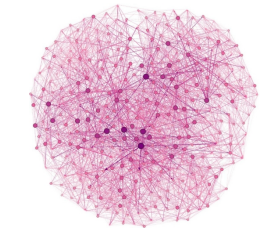
\includegraphics[width=0.5\linewidth]{imagenes/red_article_N_a.png}
    \caption{Imagen obtenida del articulo, donde se muestra la red formada de los partidos de la temporada 2023-2024}
    \label{fig:red_article}
\end{figure}
En el articulo tambien se analiza los pases que hay en la WNBA (Como la figura \ref{fig:pases_article}), dividen la cancha en 28 regiones donde se representan cada pase, como desventaja no se puede identificar que jugadora realizo el pase, solo identifican regiones dentro de la cancha, ademas de que esta red de pases fue construida atraves de 3 partidos, limitando el cmportamiento de la variedad de equipos que se encuentran presentes en la WNBA, lo que les limito la capacidad predictiva para la formacion de pases.
\begin{figure}[H]
    \centering
    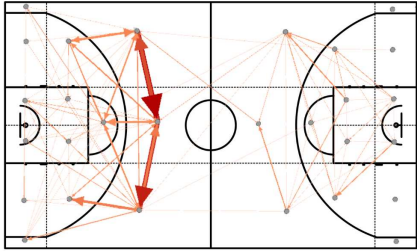
\includegraphics[width=0.5\linewidth]{imagenes/imagen_red_articulo_N_a.png}
    \caption{Imagen obtenida del articulo, en ella se muestran los pases de 3 partidos, mostrando las 28 regiones mas usuales}
    \label{fig:pases_article}
\end{figure}

Este articulo ayuda a identificar una metodologia util, para extraer informacion, que no esta presente en estadisticas tradicionales, sinembargo el conjunto de datos limitados usado representa una limitante en la aplicacion de la seleccion de alineaciones.


\cite{bonato2026networkanalysislinkprediction}

% {Descripción del TT, características, ventajas, desventajas.}
\section{Articulo: Hypergraph adjusted plus-minus}
El artículo \textit{Hypergraph adjusted plus-minus}, desarrollado por Josephs y Upton (2025), se centra en evaluar el rendimiento de los jugadores de baloncesto considerando tanto sus contribuciones individuales como las interacciones que existen entre diferentes combinaciones de jugadores. Los autores plantean que las estadísticas tradicionales no siempre permiten identificar el verdadero impacto de un jugador, debido a que su rendimiento puede depender de los compañeros con los que comparte la cancha.

Uno de los problemas que aborda el estudio es que el indicador \textit{plus-minus} (PM), que representa la diferencia entre los puntos anotados y recibidos mientras un jugador se encuentra en cancha, puede verse afectado por las sustituciones y las alineaciones utilizadas durante los partidos. Por ejemplo, un jugador puede presentar un diferencial positivo debido a que comparte una gran cantidad de minutos con compañeros de alto rendimiento, sin que necesariamente su contribución individual sea igual de importante.

Para reducir este problema, existen métodos como el \textit{Adjusted Plus-Minus} (APM), que utiliza regresión para estimar la contribución individual de cada jugador considerando a sus compañeros. Sin embargo, los autores señalan que este enfoque no representa directamente las interacciones que existen entre parejas, tríos o alineaciones completas.

En el estudio utilizaron datos \textit{play-by-play} de la NBA correspondientes a las temporadas comprendidas entre 2012 y 2022. A partir de estos datos calcularon el diferencial de puntos de las alineaciones y el tiempo que permanecieron juntas durante los partidos. Para el análisis consideraron jugadores con al menos 10,000 segundos de participación durante una temporada, con el propósito de contar con información suficiente para evaluar sus contribuciones.

Para representar las relaciones entre jugadores, los autores hacen uso de hipergrafos, una extensión de los grafos tradicionales donde una conexión puede relacionar a más de dos nodos. En este caso, los nodos representan a los jugadores y las hiperaristas representan las diferentes combinaciones que pueden formar una alineación.

A partir de esta representación proponen dos métodos para evaluar el rendimiento de las combinaciones de jugadores:

\begin{itemize}
    \item \textit{Hypergraph Adjusted Plus-Minus} (HAPM): utiliza regresión Ridge ponderada y una representación extendida de las alineaciones para estimar las contribuciones de los jugadores y clasificar combinaciones de diferentes tamaños.

    \item \textit{Line Graph Adjusted Plus-Minus} (LAPM): utiliza regresión bayesiana y la estructura de un grafo de líneas para estimar el rendimiento de las combinaciones, considerando las relaciones que existen entre ellas.
\end{itemize}

Una de las características del modelo LAPM es que utiliza la similitud de Jaccard para establecer qué tan relacionadas están dos combinaciones de jugadores. Esto permite representar la cantidad de integrantes que comparten diferentes alineaciones y utilizar esta información dentro del modelo.

Para evaluar los métodos propuestos, los autores compararon sus resultados con métricas utilizadas en el análisis de jugadores de la NBA, como \textit{Box Plus-Minus} (BPM), \textit{Player Efficiency Rating} (PER), \textit{Value Over Replacement Player} (VORP) y \textit{Win Shares per 48 minutes} (WS/48).

Los resultados muestran que HAPM presenta una mayor concordancia que el APM tradicional con algunas métricas avanzadas, como BPM, PER y VORP. Por otra parte, LAPM presenta una relación favorable con WS/48. También realizaron pruebas utilizando información de la primera mitad de una temporada para evaluar el comportamiento observado durante la segunda mitad, donde LAPM obtuvo los mejores resultados de correlación en las comparaciones presentadas.

Como ejemplo de aplicación, analizaron a los Philadelphia 76ers durante la temporada 2021--2022, identificando las contribuciones individuales y las combinaciones de parejas y tríos. Entre los resultados encontraron que la combinación de James Harden y Joel Embiid presentó un rendimiento favorable, incluso cuando ambos jugadores compartieron una cantidad limitada de minutos durante la temporada. Este análisis permitió identificar combinaciones cuyo rendimiento no resultaba tan evidente al observar únicamente el diferencial de puntos tradicional.

Una de las principales ventajas del estudio es que permite evaluar simultáneamente jugadores individuales y combinaciones de diferentes tamaños, en lugar de limitar el análisis a las alineaciones completas de cinco jugadores. Esto proporciona información adicional sobre las interacciones entre compañeros y permite identificar grupos que pueden presentar un rendimiento favorable.

Otra ventaja es que los modelos propuestos consideran las relaciones existentes entre las diferentes combinaciones de jugadores. En particular, LAPM aprovecha la estructura de un grafo para relacionar alineaciones que comparten integrantes. Además, los métodos permiten generar clasificaciones de las combinaciones, las cuales pueden utilizarse para analizar posibles rotaciones dentro de un equipo.

Sin embargo, una de las principales limitaciones es que HAPM y LAPM no incorporan directamente la identidad de los jugadores del equipo contrario. Aunque los autores consideran el diferencial entre puntos anotados y recibidos, sus modelos propuestos se calculan a nivel de equipo, por lo que no representan de manera explícita los emparejamientos con los jugadores rivales.

Otra limitación es que los modelos utilizan principalmente información derivada del diferencial de puntos, sin incorporar directamente características individuales como el estilo de juego, las habilidades ofensivas y defensivas o las funciones que desempeña cada jugador. Esto puede dificultar la interpretación de las razones por las que una combinación obtiene mejores resultados que otra.

Además, los autores mencionan que existen aspectos de la preparación de los datos que pueden mejorarse, como el seguimiento del diferencial de puntos durante determinadas sustituciones realizadas en tiros libres. También señalan que podrían investigarse otras medidas de similitud entre combinaciones y diferentes estrategias para seleccionar los parámetros de regularización de sus modelos.

Este artículo representa una referencia importante para el presente proyecto, debido a que muestra cómo las interacciones entre jugadores pueden analizarse mediante estructuras de grafos y métodos estadísticos. En particular, permite comprender que el rendimiento colectivo no depende únicamente de las estadísticas individuales, sino también de las combinaciones que se forman durante los partidos. Sin embargo, el presente trabajo busca incorporar perfiles de las jugadoras de la WNBA, evaluar el rendimiento ofensivo y defensivo y considerar las características del equipo contrario, con la finalidad de estimar qué alineaciones pueden resultar más favorables dependiendo del contexto del encuentro.

\cite{josephs2025hypergraphadjustedplusminus}
\section{Articulo: Offensive Lineup Analysis in Basketball with Clustering Players Based on Shooting Style and Offensive Role}
El artículo \textit{Offensive Lineup Analysis in Basketball with Clustering Players Based on Shooting Style and Offensive Role}, desarrollado por Yamada y Fujii (2024), se centra en analizar la compatibilidad entre jugadores de baloncesto a partir de sus estilos de tiro y las funciones ofensivas que desempeñan dentro de la cancha. Los autores plantean que el rendimiento ofensivo de un equipo no depende únicamente de contar con buenos anotadores, sino también de identificar qué tipos de jugadores se complementan mejor al formar una alineación.

Para realizar este análisis utilizan dos enfoques diferentes. El primero consiste en clasificar a los jugadores según sus estilos de tiro, mientras que el segundo busca identificar sus roles ofensivos a partir de las acciones que realizan durante los partidos. Posteriormente, utilizan estas clasificaciones para evaluar la eficiencia de las combinaciones de jugadores.

En el análisis de estilos de tiro utilizaron datos de seguimiento espacial (\textit{tracking}) de 630 partidos de la temporada 2015--2016 de la NBA, considerando un total de 41,160 lanzamientos. De cada tiro extrajeron 17 características relacionadas con la posición del jugador, la distancia al aro, el desplazamiento y el tiempo que mantiene el balón antes de realizar el lanzamiento.

Para reducir la cantidad de variables utilizaron el análisis de componentes principales (PCA), pasando de 17 características a 9 dimensiones. Después calcularon la distancia de Wasserstein para comparar las distribuciones de tiros de los jugadores y aplicaron agrupamiento jerárquico mediante el método de Ward. Como resultado de este procedimiento identificaron 13 grupos de jugadores con diferentes estilos de tiro.

Para el segundo enfoque utilizaron estadísticas ofensivas de las temporadas 2015--2016 hasta 2022--2023 de la NBA. En este caso analizaron diferentes tipos de jugadas, como:

\begin{itemize}
    \item Jugadas de aislamiento (\textit{Isolation}).
    \item Bloqueos directos (\textit{Pick-and-roll}).
    \item Jugadas de transición (\textit{Transition}).
    \item Lanzamientos tras recepción (\textit{Spot-up}).
    \item Movimientos sin balón (\textit{Off-screen}).
    \item Jugadas cercanas al aro (\textit{Post-up}).
\end{itemize}

Inicialmente aplicaron el algoritmo K-means para agrupar a los jugadores según sus características ofensivas. Sin embargo, identificaron que algunos jugadores podían desempeñar diferentes funciones durante un partido y que asignarlos a una sola categoría no representaba completamente su estilo de juego.

Para resolver este problema utilizaron el algoritmo \textit{Fuzzy C-means}, que permite que un jugador pertenezca a diferentes grupos con distintos grados de pertenencia. De esta manera obtuvieron 10 grupos de roles ofensivos, considerando que un mismo jugador puede combinar características de diferentes estilos de juego.

Una vez construidos los perfiles, los autores analizaron la eficiencia de las alineaciones utilizando el indicador \textit{Offensive Rating} (OFFRTG), que representa los puntos anotados por cada 100 posesiones. Para estudiar las combinaciones de cinco jugadores utilizaron modelos de aprendizaje automático, mientras que para evaluar la compatibilidad entre parejas de estilos ofensivos emplearon modelos bayesianos.

Los resultados muestran que ciertas combinaciones de estilos de juego tienen una relación positiva con la eficiencia ofensiva del equipo. Por ejemplo, se identificaron combinaciones favorables entre jugadores que pueden generar oportunidades de anotación y aquellos que se especializan en lanzamientos exteriores o en facilitar la circulación del balón. Por otra parte, algunas combinaciones de jugadores con funciones ofensivas similares presentaron efectos menos favorables.

Una de las principales ventajas de este estudio es que no utiliza únicamente las posiciones tradicionales de los jugadores, como base, escolta, alero o pívot, sino que construye perfiles a partir de sus características y acciones ofensivas. Esto permite identificar diferencias entre jugadores que ocupan una misma posición, pero que desempeñan funciones distintas durante el partido.

Otra ventaja es el uso de \textit{Fuzzy C-means}, ya que permite representar jugadores con características híbridas, evitando que cada uno tenga que pertenecer obligatoriamente a una sola categoría. Además, el uso de modelos bayesianos permite cuantificar los efectos de las combinaciones de estilos ofensivos y comparar cuáles presentan relaciones más favorables con el rendimiento del equipo.

Sin embargo, la principal limitación del artículo es que se centra únicamente en la eficiencia ofensiva, dejando de lado el impacto defensivo de los jugadores y de las alineaciones. Esto es importante debido a que una combinación puede producir una gran cantidad de puntos, pero también permitir que el equipo contrario anote con facilidad.

Otra limitación es que el análisis de estilos de tiro utiliza datos de seguimiento de una sola temporada, mientras que el análisis de roles ofensivos considera varias temporadas. Además, las combinaciones se evalúan principalmente a partir de los estilos de los jugadores, sin estudiar de manera directa cómo estos se comportan frente a las características particulares de una alineación rival.

También se debe considerar que los autores analizan la compatibilidad entre grupos de estilos de juego, por lo que los resultados no necesariamente representan el rendimiento específico de una pareja de jugadores. Dos jugadores pueden pertenecer a categorías similares y presentar resultados diferentes debido a sus capacidades individuales.

Este artículo proporciona una metodología útil para el presente proyecto, principalmente en la construcción de perfiles de jugadoras mediante técnicas de aprendizaje automático. La clasificación de las jugadoras según sus características ofensivas puede servir como referencia para identificar patrones y posteriormente evaluar diferentes combinaciones. Sin embargo, el proyecto busca ampliar este enfoque considerando tanto el rendimiento ofensivo como el defensivo, además de incorporar las características del equipo contrario para estimar las alineaciones más convenientes en diferentes situaciones del partido.

 \cite{yamada2024offensivelineupanalysisbasketball}.

\section{Articulo: Identifying group contributions in NBA lineups with spectral analysis}
El artículo \textit{Identifying group contributions in NBA lineups with spectral analysis}, desarrollado por Devlin y Uminsky (2020), se centra en analizar cómo las diferentes combinaciones de jugadores contribuyen al rendimiento de un equipo de baloncesto. Los autores plantean que las estadísticas individuales no siempre representan el impacto real que tiene un jugador dentro de la cancha, ya que su rendimiento también depende de los compañeros con los que comparte una alineación.

El estudio utiliza datos \textit{play-by-play} de la temporada 2015--2016 de la NBA, tomando como referencia los 15 jugadores de cada equipo con mayor número de posesiones disputadas. A partir de estos datos calculan el indicador \textit{plus-minus}, que representa el diferencial entre los puntos anotados y recibidos por una alineación durante su participación. Considerando una plantilla de 15 jugadores, existen 3003 combinaciones posibles de cinco jugadores, aunque muchas de ellas no llegan a presentarse durante los partidos.

Para analizar estas combinaciones, los autores hacen uso del análisis espectral, una técnica matemática que permite separar las contribuciones al rendimiento del equipo dependiendo del número de jugadores que participan en una combinación. De esta manera, el rendimiento se divide en diferentes niveles:

\begin{itemize}
    \item Contribución individual de cada jugador.
    \item Contribución de parejas de jugadores.
    \item Contribución de grupos de tres jugadores.
    \item Contribución de grupos de cuatro jugadores.
    \item Contribución de alineaciones completas de cinco jugadores.
\end{itemize}

Una de las principales ventajas de este método es que permite identificar si el buen rendimiento de una combinación se debe a la calidad individual de sus integrantes o a la interacción que existe entre ellos. Por ejemplo, una pareja puede presentar buenos resultados porque uno de sus jugadores tiene un rendimiento individual elevado, sin que necesariamente exista una contribución positiva adicional por jugar juntos. El análisis espectral permite distinguir estas contribuciones mediante una descomposición ortogonal.

En los resultados se analizaron las contribuciones de diferentes grupos de jugadores de los Golden State Warriors y los Boston Celtics durante la temporada estudiada. Los autores muestran que algunas combinaciones presentan un rendimiento diferente al que se podría esperar observando únicamente sus estadísticas individuales. Esto permite identificar grupos con interacciones favorables y también combinaciones cuyo rendimiento se explica principalmente por las capacidades individuales de sus integrantes.

Como ventaja, este estudio permite evaluar la interacción entre jugadores sin limitarse únicamente a las alineaciones completas de cinco integrantes. Además, proporciona información para analizar posibles rotaciones, ya que permite identificar parejas o grupos que presentan buenas contribuciones colectivas. Otra característica importante es que no necesita clasificar previamente a los jugadores según su posición o estilo de juego, debido a que las contribuciones se obtienen directamente del rendimiento observado de las alineaciones.

Sin embargo, una de sus limitaciones es que el análisis se realiza a partir de datos históricos y del rendimiento que tuvieron las combinaciones durante los partidos. Por esta razón, los resultados no representan necesariamente el comportamiento que tendrán esas mismas combinaciones en encuentros posteriores. Además, el método no considera directamente características del equipo contrario, como las jugadoras rivales que se encuentran en cancha, ni otras condiciones que pueden modificar el rendimiento de una alineación.

Otra limitación es que las combinaciones de jugadores no participan durante la misma cantidad de posesiones. Algunas alineaciones tienen una gran cantidad de información disponible, mientras que otras aparecen pocas veces, lo que dificulta la comparación de sus contribuciones. Aunque los autores utilizan medidas que consideran el número de posesiones para facilitar el análisis, esta diferencia continúa siendo una característica importante de los datos utilizados.

Este artículo resulta relevante para el presente proyecto debido a que demuestra que el rendimiento de una alineación no depende solamente de la suma de las capacidades individuales de las jugadoras, sino también de las interacciones que existen entre ellas. Sin embargo, a diferencia de este enfoque, se busca considerar las características individuales de las jugadoras de la WNBA, el rendimiento ofensivo y defensivo y la información del equipo contrario para estimar qué combinaciones pueden resultar más favorables durante un encuentro.

\section{Tabla comparativa}
En la Tabla~\ref{tab:comparativa} se presenta una
comparación de las principales características
de los trabajos analizados, considerando los
métodos utilizados, el análisis de jugadores
y alineaciones, así como las variables que
se consideran para evaluar su rendimiento.

\begin{table}[htbp]
    \centering
    \caption{Tabla comparativa de los trabajos analizados}
    \label{tab:comparativa}
    \small
    \setlength{\tabcolsep}{4pt}
    \renewcommand{\arraystretch}{1.3}

    \begin{tabular}{p{4.3cm}ccccccc}
        \toprule
        \textbf{Trabajo} &
        \textbf{C1} &
        \textbf{C2} &
        \textbf{C3} &
        \textbf{C4} &
        \textbf{C5} &
        \textbf{C6} &
        \textbf{C7} \\
        \midrule

        Chen et al. \cite{Chen17122023}
        & -- & \checkmark & \checkmark
        & \checkmark & -- & \checkmark
        & $\triangle$ \\

        Bonato y Hinds
        \cite{bonato2026networkanalysislinkprediction}
        & $\triangle$ & -- & --
        & \checkmark & $\triangle$ & --
        & $\triangle$ \\

        Josephs y Upton
        \cite{josephs2025hypergraphadjustedplusminus}
        & \checkmark & \checkmark & --
        & \checkmark & \checkmark & $\triangle$
        & -- \\

        Yamada y Fujii
        \cite{yamada2024offensivelineupanalysisbasketball}
        & \checkmark & \checkmark & \checkmark
        & \checkmark & \checkmark & --
        & -- \\

        Devlin y Uminsky
        \cite{devlin2020identifyinggroupcontributionsnba}
        & \checkmark & \checkmark & --
        & -- & \checkmark & $\triangle$
        & -- \\

        \midrule

        \textbf{Propuesta}
        &  &  & 
        &  &  & 
        & \\

        \bottomrule
    \end{tabular}
\end{table}

Las características consideradas para la
comparación son las siguientes:

\begin{itemize}
    \item[C1.] Analiza el rendimiento individual
    de los jugadores.

    \item[C2.] Analiza combinaciones de jugadores
    o alineaciones completas.

    \item[C3.] Utiliza técnicas de clustering
    para clasificar jugadores o alineaciones.

    \item[C4.] Utiliza modelos estadísticos o de
    aprendizaje automático para estimar el
    rendimiento.

    \item[C5.] Considera las interacciones entre
    jugadores de una misma alineación.

    \item[C6.] Considera el rendimiento ofensivo
    y defensivo.

    \item[C7.] Considera las características
    o emparejamientos del equipo contrario
    para evaluar alineaciones.
\end{itemize}

La simbología utilizada en la tabla es:

\begin{itemize}
    \item[$\checkmark$] La característica
    está considerada en el estudio.

    \item[$\triangle$] La característica
    está considerada parcialmente.

    \item[--] La característica no se
    aborda directamente.
\end{itemize}

A partir de la Tabla~\ref{tab:comparativa},
se observa que los trabajos analizados presentan
diferentes enfoques para evaluar el rendimiento
de los jugadores y sus alineaciones. Algunos
estudios se centran en clasificar jugadores
mediante técnicas de agrupamiento, mientras
que otros analizan las contribuciones individuales
y las interacciones entre compañeros mediante
modelos estadísticos y representaciones de grafos.

Sin embargo, los enfoques revisados no integran
de manera conjunta la caracterización de las
jugadoras, el análisis de las combinaciones,
la evaluación ofensiva y defensiva y los
emparejamientos frente al equipo contrario.


% {Breve conclusión de la comparativa. Máximo un párrafo.}

% ============================================================
% CAPÍTULO 3. MARCO TEÓRICO
% ============================================================
\chapter{Marco Teórico}
% {Este capítulo debe abarcar el 35\% del documento final. Solo definiciones,
%  no análisis. Redactar con base en varias fuentes, referenciadas.}
\section{Web Scraping}
Web Scrapping es la practica donde se recopilan datos, por cualquier medio que no sea una API o ser humano haciendo uso de un navegador web. Es un programa que tras leer codigo HTML y otros archivos que forman parte de una pagina web, solicita los datos y extrae la informacion requerida.\cite{mitchell2015web}
\section{Criptografía}
De acuerdo con \cite{ejemploX} la palabra criptografía proviene del latín \ldots

\subsection{Algoritmos criptográficos}
Según \cite{ejemploZ} se pueden clasificar los algoritmos \ldots

\subsubsection{DES}
El primer algoritmo criptográfico, de acuerdo con \cite{ejemploY}, es \ldots

\section{Lenguaje de programación}
En \cite{ejemploW} se define a un lenguaje de programación como \ldots

% ============================================================
% CAPÍTULO 4. ANÁLISIS
% ============================================================
\chapter{Análisis}
El capítulo describe los recursos analíticos, el modelo de datos previsto y la factibilidad del trabajo. El alcance es exclusivamente el desarrollo y evaluación de un modelo, no la construcción de un sistema de software.

\section{Herramientas y modelos a utilizar}
El proyecto se centra en el diseño, entrenamiento y evaluación de un modelo de recomendación de quintetos; no contempla desarrollar una aplicación informática para usuarios finales. Las herramientas se seleccionan por su utilidad para preparar datos, comparar métodos y reproducir los experimentos.

\begin{itemize}
 \item \textbf{Python:} lenguaje propuesto para integrar conjuntos tabulares y ejecutar los experimentos.
 \item \textbf{Pandas y PyArrow:} bibliotecas para consultar, transformar y almacenar archivos Parquet.
 \item \textbf{Scikit-learn:} biblioteca candidata para normalización, agrupamiento, modelos de referencia y evaluación.
 \item \textbf{Herramientas estadísticas:} técnicas de regularización y estimación de efectos de jugadoras o quintetos, cuya implementación específica se decidirá tras la exploración de datos.
 \item \textbf{Optimización combinatoria:} búsqueda y comparación de quintetos factibles mediante una función de desempeño estimado.
\end{itemize}

Se compararán métodos de agrupamiento para perfiles \textit{Guard}, \textit{Wing} y \textit{Big}, modelos predictivos del rendimiento colectivo y un optimizador que seleccione las cinco jugadoras disponibles. No se considera ninguno de estos métodos como implementado o validado en esta etapa. La fuente principal propuesta para las estadísticas es wehoop \cite{wehoopRepositorio}, cuya estructura y limitaciones se describen en el modelo de datos.

\section{Modelo de datos}
\subsection{Fuentes de información}
La fuente principal propuesta es el repositorio público \textit{wehoop-wnba-stats-data}, que contiene registros procesados de WNBA Stats. Las familias relevantes se relacionan en la Tabla~\ref{tab:fuentes_wehoop}. La disponibilidad de carpetas no garantiza igual cobertura ni completitud en todas las temporadas.
\begin{table}[htbp]\centering\small
\caption{Fuentes de datos y aplicación propuesta.}\label{tab:fuentes_wehoop}
\begin{tabularx}{\textwidth}{@{}p{3.1cm}XX@{}}\toprule
\textbf{Conjunto} & \textbf{Información} & \textbf{Uso en el modelo}\\\midrule
\texttt{pbp} & Eventos, periodo, reloj, marcador y persona asociada. & Contexto temporal de las acciones.\\
\texttt{game\_lineups} & Alineaciones por partido; esquema por verificar. & Reconstrucción de quintetos.\\
\texttt{possessions} & Registros de posesiones; esquema por verificar. & Normalización por posesiones.\\
\texttt{lineups} & Métricas agregadas de alineaciones. & Referencia de rendimiento colectivo.\\
\texttt{player\_season\_stats} & Estadísticas individuales por temporada. & Perfiles funcionales.\\
\texttt{player\_game\_logs} & Estadísticas por encuentro y jugadora. & Características históricas.\\
\texttt{shots} & Tiros y posiciones de lanzamiento. & Estilos de anotación.\\
\texttt{game\_rosters} & Plantillas por partido. & Identificación de participantes.\\
\bottomrule\end{tabularx}\end{table}
La documentación de metadatos puede consultarse en \url{https://github.com/sportsdataverse/wehoop-wnba-stats-data/tree/main/docs/datasets}. Se verificará cada esquema Parquet antes de construir el conjunto de entrenamiento.
\subsection{Diccionario de datos originales}
La Tabla~\ref{tab:campos_wehoop} contiene nombres y tipos efectivamente documentados por wehoop. No representa todas las columnas posibles ni valida valores de cada archivo Parquet.
\begin{longtable}{@{}p{3cm}p{3cm}p{2cm}p{5cm}@{}}
\caption{Campos de origen documentados.}\label{tab:campos_wehoop}\\
\toprule\textbf{Campo}&\textbf{Conjunto}&\textbf{Tipo}&\textbf{Descripción}\\\midrule\endfirsthead
\toprule\textbf{Campo}&\textbf{Conjunto}&\textbf{Tipo}&\textbf{Descripción}\\\midrule\endhead
\texttt{game\_id}&\texttt{pbp}&String&Identificador textual de partido.\\
\texttt{season}&\texttt{pbp}&Int64&Temporada WNBA.\\
\texttt{period}&\texttt{pbp}&Int64&Periodo o prórroga.\\
\texttt{clock}&\texttt{pbp}&String&Reloj del evento en ISO 8601.\\
\texttt{action\_number}&\texttt{pbp}&Int64&Orden de la acción.\\
\texttt{team\_id}&\texttt{pbp}&Int64&Identificador de equipo.\\
\texttt{person\_id}&\texttt{pbp}&Int64&Persona vinculada a la acción.\\
\texttt{action\_type}&\texttt{pbp}&String&Tipo de acción.\\
\texttt{score\_home}&\texttt{pbp}&String&Marcador local.\\
\texttt{score\_away}&\texttt{pbp}&String&Marcador visitante.\\
\texttt{x\_legacy}&\texttt{shots}&Int64&Coordenada de tiro.\\
\texttt{y\_legacy}&\texttt{shots}&Int64&Coordenada de tiro.\\
\texttt{shot\_result}&\texttt{shots}&String&Resultado de lanzamiento.\\
\texttt{player\_id}&\texttt{player\_season\_stats}&Int64&ID de jugadora.\\
\texttt{age}&\texttt{player\_season\_stats}&Float64&Edad.\\
\texttt{ts\_pct}&\texttt{player\_season\_stats}&Float64&Eficiencia de tiro.\\
\texttt{usg\_pct}&\texttt{player\_season\_stats}&Float64&Uso ofensivo.\\
\texttt{off\_rating}&\texttt{lineups}&Float64&Rating ofensivo agregado.\\
\texttt{def\_rating}&\texttt{lineups}&Float64&Rating defensivo agregado.\\
\texttt{net\_rating}&\texttt{lineups}&Float64&Rating neto agregado.\\
\texttt{poss}&\texttt{lineups}&Int64&Posesiones.\\
\texttt{player\_id}&\texttt{game\_rosters}&Int64&ID en plantilla del partido.\\
\bottomrule\end{longtable}
Los ratings de \texttt{lineups} no deben interpretarse automáticamente como rendimientos de enfrentamientos entre dos quintetos específicos. Las coordenadas de tiro tampoco identifican a la defensora.
\subsection{Variables derivadas para el modelo}
Las tablas siguientes contienen \textbf{variables que se propone construir}, no columnas originales documentadas en wehoop.
\begin{longtable}{@{}p{3.6cm}p{2cm}p{6.5cm}@{}}
\caption{Variables derivadas de intervalos de alineación.}\label{tab:stints_wnba}\\
\toprule\textbf{Campo}&\textbf{Tipo}&\textbf{Construcción}\\\midrule\endfirsthead
\toprule\textbf{Campo}&\textbf{Tipo}&\textbf{Construcción}\\\midrule\endhead
\texttt{stint\_id}&Texto&Identificador generado por intervalo sin cambios de quinteto.\\
\texttt{start\_clock}&Tiempo&Inicio del intervalo.\\
\texttt{end\_clock}&Tiempo&Fin del intervalo.\\
\texttt{stint\_seconds}&Decimal&Duración calculada dentro del periodo.\\
\texttt{home\_team\_id}&ID&Equipo local, enlazado con los datos del partido.\\
\texttt{away\_team\_id}&ID&Equipo visitante.\\
\texttt{score\_margin\_start}&Entero&Diferencial al inicio.\\
\texttt{score\_margin\_end}&Entero&Diferencial al final.\\
\texttt{focal\_lineup}&Conjunto&Cinco jugadoras propias, si es reconstruible.\\
\texttt{opponent\_lineup}&Conjunto&Cinco rivales, si es reconstruible.\\
\bottomrule\end{longtable}
\begin{longtable}{@{}p{3.6cm}p{2cm}p{6.5cm}@{}}
\caption{Variables derivadas de coincidencia contextual entre rivales.}\label{tab:coincidencias_wnba}\\
\toprule\textbf{Campo}&\textbf{Tipo}&\textbf{Construcción}\\\midrule\endfirsthead
\toprule\textbf{Campo}&\textbf{Tipo}&\textbf{Construcción}\\\midrule\endhead
\texttt{focal\_player\_id}&ID&Jugadora propia presente en el intervalo.\\
\texttt{opponent\_player\_id}&ID&Rival simultáneamente presente, no defensora demostrada.\\
\texttt{focal\_role}&Categoría&Perfil estimado Guard, Wing o Big.\\
\texttt{opponent\_role}&Categoría&Perfil estimado de la rival.\\
\texttt{compatible\_roles}&Binario&Regla de compatibilidad por validar.\\
\texttt{focal\_starter}&Binario&Titularidad inferida o verificada.\\
\texttt{opponent\_starter}&Binario&Titularidad rival.\\
\texttt{shared\_seconds}&Decimal&Segundos de coincidencia.\\
\texttt{shared\_possessions}&Entero&Posesiones durante coincidencia reconstruidas.\\
\texttt{focal\_off\_possessions}&Entero&Posesiones ofensivas coincidentes.\\
\texttt{focal\_def\_possessions}&Entero&Posesiones defensivas coincidentes.\\
\texttt{shared\_seconds\_game}&Decimal&Segundos compartidos en el partido.\\
\texttt{shared\_possessions\_game}&Entero&Posesiones compartidas en el partido.\\
\bottomrule\end{longtable}
Las estadísticas de puntos, tiros, rebotes, asistencias, pérdidas, robos, bloqueos y faltas durante cada coincidencia requerirán agregación de acciones verificables; no corresponden a los totales de temporada.
\subsection{Validación y limitaciones de los datos}
\subsubsection{Cobertura y consistencia}
Se comprobarán temporadas, cobertura de partidos, nombres y tipos de columnas Parquet, valores faltantes, claves y duplicados. Las uniones utilizarán identificadores documentados como \texttt{game\_id}, \texttt{team\_id} y \texttt{player\_id}/\texttt{person\_id}. La reconstrucción de intervalos sin sustituciones y de posesiones se contrastará con marcadores y estadísticas agregadas.

Se validará cronológicamente: para pronosticar un partido se usarán exclusivamente datos disponibles antes de ese partido, evitando fuga de información procedente del final de temporada. Se indicará el tamaño de muestra y se excluirán o suavizarán exposiciones demasiado pequeñas.

\subsubsection{Alcance de las comparaciones individuales}
Las coordenadas de tiro no equivalen a \textit{tracking} espacial continuo. La coincidencia de rivales en cancha no demuestra que una defendió directamente a otra; el modelo analizará \emph{comparaciones contextuales durante minutos compartidos}.

\section{Análisis de factibilidad}
\subsection{Factibilidad técnica}
La factibilidad técnica depende de disponer de registros suficientes para identificar jugadoras, encuentros y eventos, así como de reconstruir intervalos donde permanezcan constantes ambos quintetos. El repositorio wehoop incluye familias de datos para eventos de juego, estadísticas individuales y plantillas \cite{wehoopRepositorio}; sin embargo, la viabilidad del análisis de enfrentamientos entre quintetos deberá comprobarse inspeccionando la granularidad y cobertura efectiva de los archivos Parquet.

El trabajo es abordable con bibliotecas de análisis de datos y modelos estadísticos disponibles para Python. La estimación de recursos de cómputo se realizará a partir del número de observaciones, variables y combinaciones factibles, sin asumir que un sistema de inferencia en tiempo real forma parte del alcance.
\subsection{Factibilidad metodológica}
La factibilidad metodológica se evaluará mediante la calidad y representatividad de las observaciones. Se plantea utilizar varias temporadas con ponderación por recencia para reducir la inestabilidad de parejas y quintetos con pocas posesiones, además de seleccionar inicialmente cinco equipos con continuidad de plantilla verificable.

La validez de los resultados dependerá de establecer particiones temporales, tamaños mínimos de muestra, referencias comparativas y métricas apropiadas de predicción y recomendación. Los quintetos observados históricamente podrían no cubrir todas las combinaciones posibles; por ello, el modelo deberá informar incertidumbre y no interpretar las predicciones de combinaciones inéditas como resultados comprobados.
\subsection{Factibilidad de datos y uso responsable}
El acceso a datos públicamente distribuidos por wehoop facilita desarrollar experimentos reproducibles \cite{wehoopRepositorio}. Se documentarán el origen y la licencia de los conjuntos utilizados, sus condiciones de redistribución y la fecha de consulta; esto no equivale a afirmar que todas las variables estén disponibles o sean libres de restricciones.

No se dispone, en las fuentes documentadas que se han seleccionado, de evidencia suficiente para identificar emparejamientos defensivos individuales continuos. Por tanto, el alcance se limitará a comparaciones contextuales de jugadoras simultáneamente presentes y a enfrentamientos colectivos entre quintetos. No se contempla la creación de un sistema comercial ni la adquisición de datos privados de seguimiento espacial.

% ============================================================
% CAPÍTULO 5. PREPROCESAMIENTO
% ============================================================
\chapter{Preprocesamiento}
\section{Etapas del preprocesamiento}
\subsection{Descripción de los datos}
Se utilizarán conjuntos de estadísticas de la WNBA publicados por el proyecto wehoop \cite{wehoopRepositorio}. La documentación distingue registros de eventos \textit{play-by-play} \cite{wehoopPbp}, estadísticas individuales por temporada \cite{wehoopPlayerSeason}, tiros \cite{wehoopShots} y métricas agregadas de alineaciones \cite{wehoopLineups}. De manera complementaria se examinarán los archivos de alineaciones por partido, posesiones, registros de encuentro y plantillas.

La unidad de observación no será única para todas las fuentes: una fila puede representar un evento, un partido, una jugadora o un resumen de alineación. Esta diferencia exige definir previamente las claves de integración y la granularidad de cada tabla. El conjunto de entrenamiento que se propone construir tendrá como unidad principal el intervalo de coincidencia entre un quinteto propio y otro rival, siempre que ambos puedan reconstruirse de forma verificable.

Las tablas del Capítulo 4 distinguen los campos publicados por la fuente y las variables derivadas que se pretenden calcular. No se asumirá que estas últimas existen como columnas nativas.
\subsection{Limpieza}
La limpieza comenzará con la inspección de los esquemas Parquet, tipos de datos, rangos y valores faltantes. Se comprobará que los identificadores de partido, equipo y jugadora sean consistentes entre las fuentes y que los registros duplicados no generen conteos incorrectos. Para los eventos de juego se revisará el orden temporal por partido y periodo y se normalizará la representación del reloj antes de calcular duraciones.

Se separarán temporadas y tipos de competición cuando el conjunto lo permita. Las métricas calculadas sobre temporadas completas no se utilizarán como predictores para fechas anteriores a su cierre. Se documentarán los criterios de exclusión por registros incompletos, intervalos ambiguos y exposición insuficiente en posesiones, conservando trazabilidad de cada transformación.

Una observación faltante no se reemplazará automáticamente por cero, pues ausencia de registro y ausencia de acción representan situaciones distintas.
\subsection{Análisis exploratorio de datos}
El análisis exploratorio permitirá describir la cobertura anual, el número de partidos y jugadoras disponibles, la distribución de minutos y posesiones, así como la frecuencia de cada quinteto y de sus enfrentamientos observados. Se estudiarán los valores extremos y la variabilidad de los ratings ofensivo, defensivo y neto para identificar estimaciones inestables por tamaño de muestra.

También se analizarán distribuciones y correlaciones de puntos, asistencias, rebotes, pérdidas, robos, bloqueos y métricas de tiro, con el propósito de seleccionar atributos adecuados para caracterizar perfiles. Las visualizaciones y resúmenes se presentarán sólo después de ejecutar la exploración; no se reportan cifras observadas en esta propuesta.
\subsection{Procesamiento}
El procesamiento integrará los eventos por identificador de partido y orden temporal con la información de plantillas, alineaciones y posesiones. Se intentará delimitar intervalos sin sustituciones, reconstruir los cinco integrantes de cada equipo y contabilizar tiempo, marcador y posesiones durante el enfrentamiento. Los intervalos cuya reconstrucción no sea inequívoca se marcarán como no verificables.

Posteriormente se derivarán estadísticas contextuales de jugadoras que coinciden en cancha y agregados colectivos por quinteto y rival. La coincidencia contextual no se confundirá con la identificación de la defensora directa. Las características históricas se calcularán con ventanas temporales anteriores a cada partido para evitar fuga de información.

Las variables derivadas se explican en las Tablas~\ref{tab:stints_wnba} y \ref{tab:coincidencias_wnba}. El conjunto procesado servirá como entrada para la comparación de técnicas de agrupamiento, estimación del rendimiento y optimización, descritas en el Capítulo 6.
\subsection{Presentación de resultados}
La presentación de resultados del preprocesamiento consistirá en describir el número de registros originales y conservados por fuente, temporada y equipo; los valores faltantes; los intervalos y posesiones reconstruidos; y las observaciones descartadas con su justificación. También se documentarán distribuciones de exposición de quintetos y ejemplos de tablas finales de entrenamiento, sin confundirlos con resultados de predicción.

Para evaluar los modelos en una etapa posterior se comunicarán tanto el \textit{Net Rating} esperado como la probabilidad de diferencial positivo, acompañados de métricas de error, calibración y ordenamiento de recomendaciones. La presentación distinguirá resultados experimentales medidos de objetivos metodológicos aún pendientes.

% ============================================================
% CAPÍTULO 6. DESARROLLO DEL MODELO
% ============================================================
% CAPÍTULO 6. DESARROLLO E IMPLEMENTACIÓN
% ============================================================
\chapter{Desarrollo y evaluación del modelo}

\section{Desarrollo del proyecto}
La primera fase integra históricos de jugadoras y de quintetos para estimar perfiles e interacciones. La ponderación entre temporadas, los métodos de regularización y los algoritmos de agrupamiento se elegirán mediante experimentos con validación temporal.

En la segunda fase se estimará el rendimiento esperado de un quinteto candidato frente a la alineación rival:
\begin{equation}
 Q_B^*=\underset{Q_B\subseteq R_B,\;|Q_B|=5}{\operatorname{arg\,max}}\widehat f(Q_B,Q_A,c),
\end{equation}
donde $R_B$ representa las jugadoras disponibles, $Q_A$ el quinteto rival y $c$ el contexto conocido antes de decidir. Se explorará la restricción de máximo una sustitución por recomendación. Las salidas serán un \textit{Net Rating} esperado y una probabilidad de diferencial positivo, evaluadas mediante error, calibración y calidad del ordenamiento.

\section{Evaluación experimental}
Se documentarán la validación temporal, los métodos de referencia y las métricas de predicción y recomendación una vez ejecutados los experimentos.

% ============================================================
% CAPÍTULO 7. PRUEBAS
% ============================================================
\chapter{Pruebas}

\section{Generación del plan de pruebas}

\begin{table}[H]
\centering
\caption{Registro de revisiones}
\begin{tabular}{@{}p{1.3cm}p{2.2cm}p{2.7cm}p{2.7cm}p{4.5cm}@{}}
\toprule
\textbf{Versión} & \textbf{Fecha} & \textbf{Autor} & \textbf{Revisor} & \textbf{Observaciones} \\
\midrule
1.0 & dd/mm/aaaa & Nombre (estudiante) & Nombre (director/a) & Desarrollo del módulo de inicio de sesión y conexión con la base de datos \\
1.1 & dd/mm/aaaa & Nombre (estudiante) & Nombre (director/a) & Desarrollo del módulo de gestión de perfil del usuario \\
\bottomrule
\end{tabular}
\end{table}

\subsection{Construcción y ejecución de pruebas}

\begin{table}[H]
\centering
\caption{Componentes probados}
\begin{tabular}{@{}ll@{}}
\toprule
\textbf{Componentes que se probaron} & \textbf{Tipo de prueba que se realizó} \\
\midrule
Módulo de registro de usuario         & Funcional \\
Módulo de inicio de sesión            & Funcional, de seguridad \\
Módulo de recuperación de contraseña  & Integral \\
\bottomrule
\end{tabular}
\end{table}

\subsection{Creación de casos y escenarios de prueba al sistema}

\begin{table}[H]
\centering
\caption{Nomenclatura de casos de prueba}
\begin{tabular}{@{}p{6.5cm}p{6.5cm}@{}}
\toprule
\textbf{Nombre del documento} & \textbf{Nombre del caso de prueba} \\
\midrule
PR-01-Pruebas\_funcionales-Inicio de sesión & PR-M/01-CU/02-Inicio de sesión \\
PR-02-Pruebas\_de\_seguridad-Inicio de sesión & PR-M/01-CU/02-Seguridad del Inicio de sesión \\
PR-03-Pruebas\_funcionales-Registro de usuario & PR-M/01-CU/01-Registro de usuarios \\
\bottomrule
\end{tabular}
\end{table}

\subsection{Ejecución de casos y escenarios de prueba al sistema}

\begin{longtable}{@{}p{2.3cm}p{3.3cm}p{2.2cm}p{1.6cm}p{2.8cm}p{1.5cm}p{1.4cm}@{}}
\toprule
\textbf{ID} & \textbf{Acción} & \textbf{Datos de entrada} & \textbf{Tipo} & \textbf{Resultado esperado} & \textbf{Resultado} & \textbf{Corrección} \\
\midrule
\endhead
PR-M/01-CU/01-ECP/01-C01 & Iniciar sesión con usuario registrado y contraseña correcta & Usuario: benji@ipn.mx / Contraseña: miPassword123 & Optimista & Mensaje de bienvenida & Correcto & NO APLICA \\
PR-M/01-CU/01-ECP/01-C02 & Iniciar sesión con usuario registrado y contraseña incorrecta & Usuario: benji@ipn.mx / Contraseña: OtroPassword789 & No Optimista & Mensaje de error, sin acceso & Correcto & NO APLICA \\
PR-M/01-CU/01-ECP/01-C03 & Iniciar sesión con usuario no registrado & Usuario: nadie@ipn.mx / Contraseña: miPassword567 & No Optimista & Mensaje de error, sin acceso & Correcto & NO APLICA \\
\bottomrule
\end{longtable}

% ============================================================
% CAPÍTULO 8. CONCLUSIONES Y TRABAJO A FUTURO
% ============================================================
\chapter{Conclusiones y trabajo a futuro}
% {Revisión reflexiva de los resultados, no un resumen del proyecto.}

% ============================================================
% REFERENCIAS (formato IEEE)
% ============================================================
\printbibliography[title={Referencias}]
\addcontentsline{toc}{chapter}{Referencias}

% ============================================================
% ANEXOS
% ============================================================
\appendix
\chapter{Anexos}
% {Contenidos complementarios que amplían la información, no imprescindibles
%  para la comprensión del proyecto (p. ej. instrumento de encuesta completo).}

\end{document}